%%===========================================================%%
%%                                                           %%
%%                  ENERGY LOSS  CORRECTION                   %%
%%                                                           %%
%%===========================================================%%


\chapter{Energy Loss Correction}\label{chap:energyLossCorrection}
Particles passing through the detector material lose energy as they travel. The track momentum $p_T$ is reconstructed by fitting a helical path to the track points left in the detector. Fitting the track points to an ideal
helical track tends to underestimate the momentum due to these energy loss effects. To minimize biases due to this effect, correction procedure is applied 
during standard track momentum reconstruction  for both data and MC simulation. For this procedure pion hypothesis is used  and the reconstructed momentum $p_T^{meas}$ is corrected by the amount of energy loss specific for a pion.  For all particles but a pion some rest bias  is still present since  energy loss is specific for each particle type. These biases  can be determined from simulated tracks run through GEANT.
The correction $p_T^{meas}-p_T^{true}$ was calculated for each particle species as a function of $p_T^{meas}$, $\eta$ and $z$-vertex. The sample energy loss correction averaged over $|\eta|<0.7$ for $K^-$ is shown in Fig. \ref{fig:energyLossPrimaryK_minus_sample}. 
\noindent The energy loss corrections for other particle species are shown in \Cref{fig:energyLossPrimaryPi_minus,fig:energyLossPrimaryPi_plus,fig:energyLossPrimaryK_minus,fig:energyLossPrimaryK_plus,fig:energyLossPrimaryP_bar,fig:energyLossPrimaryP,fig:energyLossPrimaryNegative,fig:energyLossPrimaryPositive,fig:energyLossPrimaryP_barGlobal,fig:energyLossPrimaryPGlobal} in Appendix \ref{appendix:energyLoss}.\newline



\begin{figure}[hb]

\centering
 \includegraphics[width=0.9\linewidth,page=30]{graphics/energyLoss/energyLoss3D_OnePrtAlso.pdf}
 \caption[Sample energy loss correction for $K^-$ as a function of reconstructed transverse momentum $p_T^{meas}$.]{Sample energy loss correction $p_T^{meas}-p_T^{true}$ for $K^-$ as a function of reconstructed transverse momentum $p_T^{meas}$ $\left(|\eta|<0.7\right)$ in single $z$-vertex bin, $-10<V_z <0$~cm. Red lines and arrows indicate region accepted in analyses.}\label{fig:energyLossPrimaryK_minus_sample}

\end{figure}